\documentclass[12pt,]{book}
\usepackage{lmodern}
\usepackage{amssymb,amsmath}
\usepackage{ifxetex,ifluatex}
\usepackage{fixltx2e} % provides \textsubscript
\ifnum 0\ifxetex 1\fi\ifluatex 1\fi=0 % if pdftex
  \usepackage[T1]{fontenc}
  \usepackage[utf8]{inputenc}
\else % if luatex or xelatex
  \ifxetex
    \usepackage{mathspec}
  \else
    \usepackage{fontspec}
  \fi
  \defaultfontfeatures{Ligatures=TeX,Scale=MatchLowercase}
    \setmonofont[Mapping=tex-ansi,Scale=0.7]{Source Code Pro}
\fi
% use upquote if available, for straight quotes in verbatim environments
\IfFileExists{upquote.sty}{\usepackage{upquote}}{}
% use microtype if available
\IfFileExists{microtype.sty}{%
\usepackage{microtype}
\UseMicrotypeSet[protrusion]{basicmath} % disable protrusion for tt fonts
}{}
\usepackage[margin=1in]{geometry}
\usepackage{hyperref}
\hypersetup{unicode=true,
            pdftitle={A Complex Systems Approach to the Behavioural Sciences},
            pdfauthor={Fred Hasselman \& Maarten Wijnants},
            pdfborder={0 0 0},
            breaklinks=true}
\urlstyle{same}  % don't use monospace font for urls
\usepackage{natbib}
\bibliographystyle{apalike}
\usepackage{color}
\usepackage{fancyvrb}
\newcommand{\VerbBar}{|}
\newcommand{\VERB}{\Verb[commandchars=\\\{\}]}
\DefineVerbatimEnvironment{Highlighting}{Verbatim}{commandchars=\\\{\}}
% Add ',fontsize=\small' for more characters per line
\usepackage{framed}
\definecolor{shadecolor}{RGB}{248,248,248}
\newenvironment{Shaded}{\begin{snugshade}}{\end{snugshade}}
\newcommand{\KeywordTok}[1]{\textcolor[rgb]{0.13,0.29,0.53}{\textbf{#1}}}
\newcommand{\DataTypeTok}[1]{\textcolor[rgb]{0.13,0.29,0.53}{#1}}
\newcommand{\DecValTok}[1]{\textcolor[rgb]{0.00,0.00,0.81}{#1}}
\newcommand{\BaseNTok}[1]{\textcolor[rgb]{0.00,0.00,0.81}{#1}}
\newcommand{\FloatTok}[1]{\textcolor[rgb]{0.00,0.00,0.81}{#1}}
\newcommand{\ConstantTok}[1]{\textcolor[rgb]{0.00,0.00,0.00}{#1}}
\newcommand{\CharTok}[1]{\textcolor[rgb]{0.31,0.60,0.02}{#1}}
\newcommand{\SpecialCharTok}[1]{\textcolor[rgb]{0.00,0.00,0.00}{#1}}
\newcommand{\StringTok}[1]{\textcolor[rgb]{0.31,0.60,0.02}{#1}}
\newcommand{\VerbatimStringTok}[1]{\textcolor[rgb]{0.31,0.60,0.02}{#1}}
\newcommand{\SpecialStringTok}[1]{\textcolor[rgb]{0.31,0.60,0.02}{#1}}
\newcommand{\ImportTok}[1]{#1}
\newcommand{\CommentTok}[1]{\textcolor[rgb]{0.56,0.35,0.01}{\textit{#1}}}
\newcommand{\DocumentationTok}[1]{\textcolor[rgb]{0.56,0.35,0.01}{\textbf{\textit{#1}}}}
\newcommand{\AnnotationTok}[1]{\textcolor[rgb]{0.56,0.35,0.01}{\textbf{\textit{#1}}}}
\newcommand{\CommentVarTok}[1]{\textcolor[rgb]{0.56,0.35,0.01}{\textbf{\textit{#1}}}}
\newcommand{\OtherTok}[1]{\textcolor[rgb]{0.56,0.35,0.01}{#1}}
\newcommand{\FunctionTok}[1]{\textcolor[rgb]{0.00,0.00,0.00}{#1}}
\newcommand{\VariableTok}[1]{\textcolor[rgb]{0.00,0.00,0.00}{#1}}
\newcommand{\ControlFlowTok}[1]{\textcolor[rgb]{0.13,0.29,0.53}{\textbf{#1}}}
\newcommand{\OperatorTok}[1]{\textcolor[rgb]{0.81,0.36,0.00}{\textbf{#1}}}
\newcommand{\BuiltInTok}[1]{#1}
\newcommand{\ExtensionTok}[1]{#1}
\newcommand{\PreprocessorTok}[1]{\textcolor[rgb]{0.56,0.35,0.01}{\textit{#1}}}
\newcommand{\AttributeTok}[1]{\textcolor[rgb]{0.77,0.63,0.00}{#1}}
\newcommand{\RegionMarkerTok}[1]{#1}
\newcommand{\InformationTok}[1]{\textcolor[rgb]{0.56,0.35,0.01}{\textbf{\textit{#1}}}}
\newcommand{\WarningTok}[1]{\textcolor[rgb]{0.56,0.35,0.01}{\textbf{\textit{#1}}}}
\newcommand{\AlertTok}[1]{\textcolor[rgb]{0.94,0.16,0.16}{#1}}
\newcommand{\ErrorTok}[1]{\textcolor[rgb]{0.64,0.00,0.00}{\textbf{#1}}}
\newcommand{\NormalTok}[1]{#1}
\usepackage{longtable,booktabs}
\usepackage{graphicx,grffile}
\makeatletter
\def\maxwidth{\ifdim\Gin@nat@width>\linewidth\linewidth\else\Gin@nat@width\fi}
\def\maxheight{\ifdim\Gin@nat@height>\textheight\textheight\else\Gin@nat@height\fi}
\makeatother
% Scale images if necessary, so that they will not overflow the page
% margins by default, and it is still possible to overwrite the defaults
% using explicit options in \includegraphics[width, height, ...]{}
\setkeys{Gin}{width=\maxwidth,height=\maxheight,keepaspectratio}
\IfFileExists{parskip.sty}{%
\usepackage{parskip}
}{% else
\setlength{\parindent}{0pt}
\setlength{\parskip}{6pt plus 2pt minus 1pt}
}
\setlength{\emergencystretch}{3em}  % prevent overfull lines
\providecommand{\tightlist}{%
  \setlength{\itemsep}{0pt}\setlength{\parskip}{0pt}}
\setcounter{secnumdepth}{5}
% Redefines (sub)paragraphs to behave more like sections
\ifx\paragraph\undefined\else
\let\oldparagraph\paragraph
\renewcommand{\paragraph}[1]{\oldparagraph{#1}\mbox{}}
\fi
\ifx\subparagraph\undefined\else
\let\oldsubparagraph\subparagraph
\renewcommand{\subparagraph}[1]{\oldsubparagraph{#1}\mbox{}}
\fi

%%% Use protect on footnotes to avoid problems with footnotes in titles
\let\rmarkdownfootnote\footnote%
\def\footnote{\protect\rmarkdownfootnote}

%%% Change title format to be more compact
\usepackage{titling}

% Create subtitle command for use in maketitle
\newcommand{\subtitle}[1]{
  \posttitle{
    \begin{center}\large#1\end{center}
    }
}

\setlength{\droptitle}{-2em}
  \title{A Complex Systems Approach to the Behavioural Sciences}
  \pretitle{\vspace{\droptitle}\centering\huge}
  \posttitle{\par}
  \author{Fred Hasselman \& Maarten Wijnants}
  \preauthor{\centering\large\emph}
  \postauthor{\par}
  \predate{\centering\large\emph}
  \postdate{\par}
  \date{2017 - 2018}

\usepackage{booktabs}
\usepackage{longtable}
\usepackage{framed,color}
\definecolor{shadecolor}{gray}{.95}
\usepackage{natbib}
\usepackage[dutch]{babel}
\usepackage{amsmath,amsfonts,amssymb}
\usepackage{graphicx}
\definecolor{shadecolor}{gray}{.95}
\usepackage{parskip}
\usepackage[margin=10pt,font=small]{caption}
\usepackage{placeins}
\usepackage{adjustbox}
\usepackage{float}
\usepackage{enumerate}
\usepackage{eso-pic}
\usepackage{everyshi}
\usepackage{bibentry}
\usepackage{changepage}
\usepackage{fontspec}
\bibpunct{(}{)}{;}{a}{,}{,}

\DeclareGraphicsExtensions{.pdf, .png, .eps, .jpg}

  \renewenvironment{quote}{%
  \par \small \medskip \block
  \leftskip=4em \rightskip=4em%
  \noindent \ignorespaces}{%
  \par \medskip
  }
 
\newcommand{\stitle}{Inleiding Wetenschappelijk Onderzoek}
\addto\captionsdutch{\renewcommand{\chaptername}{Hoofdstuk}}

% Headers
\usepackage{fancyhdr}
\pagestyle{fancy}
\fancyhf{}
\fancyhead[LE]{\nouppercase{\rightmark}}
\fancyhead[RO]{\textsc{\stitle}}
\fancyfoot[LE,RO]{\thepage}
\fancyheadoffset[RE,LO]{\textwidth}

% Create some reference defaults 
\captionsetup[figure]{labelfont=bf,labelsep=endash}
\captionsetup[table]{textfont=it,labelsep=newline}
\renewcommand{\thefigure}{\textbf{\arabic{chapter}.\arabic{figure}}}
\renewcommand{\thetable}{\textbf{\arabic{chapter}.\arabic{table}}}
%\renewcommand{\thechapter}{\textsc}

\let\stdsection\section
\renewcommand\section{\newpage\stdsection}

\setmainfont{Calibri}
\newfontface\itGS{Gill Sans Light Italic}
\newfontface\bfGS{Gill Sans SemiBold}
\newfontfamily\block{Gill Sans Light}

\ifxetex
  \usepackage{letltxmacro}
  \setlength{\XeTeXLinkMargin}{1pt}
  \LetLtxMacro\SavedIncludeGraphics\includegraphics
  \def\includegraphics#1#{% #1 catches optional stuff (star/opt. arg.)
    \IncludeGraphicsAux{#1}%
  }%
  \newcommand*{\IncludeGraphicsAux}[2]{%
    \XeTeXLinkBox{%
      \SavedIncludeGraphics#1{#2}%
    }%
  }%
\fi

\setkeys{Gin}{width=\linewidth}

\newenvironment{rmdblock}[1]
  {\begin{shaded*}
  \begin{itemize}
  \renewcommand{\labelitemi}{
    \raisebox{-.7\height}[0pt][0pt]{
      {\setkeys{Gin}{width=3em,keepaspectratio}\includegraphics{images/#1}}
    }
  }
  \item
  }
  {
  \end{itemize}
  \end{shaded*}
  }
  
\newenvironment{rmdnote}
  {\begin{rmdblock}{note}}
  {\end{rmdblock}}
\newenvironment{rmdselfThink}
  {\begin{rmdblock}{selfThink}}
  {\end{rmdblock}}
\newenvironment{rmdimportant}
  {\begin{rmdblock}{important}}
  {\end{rmdblock}}
\newenvironment{rmdkennen}
  {\begin{rmdblock}{kennen}}
  {\end{rmdblock}}
\newenvironment{rmdentertain}
  {\begin{rmdblock}{entertain}}
  {\end{rmdblock}}
\newenvironment{rmdfilo}
  {\begin{rmdblock}{Filosoof_150px}}
  {\end{rmdblock}}
\newenvironment{rmdempi}
  {\begin{rmdblock}{Empirist_150px}}
  {\end{rmdblock}}
\newenvironment{rmdscip}
  {\begin{rmdblock}{Sci-Pract_150px}}
  {\end{rmdblock}}
  
 \usepackage{hyperref}
\hypersetup{unicode=true,
            pdftitle={Inleiding Wetenschappelijk Onderzoek},
            pdfauthor={Fred Hasselman},
            pdfborder={0 0 0},
            breaklinks=true,
            colorlinks=true,
            allcolors=[rgb]{.05 .5 .7}}

\usepackage{amsthm}
\newtheorem{theorem}{Theorem}[chapter]
\newtheorem{lemma}{Lemma}[chapter]
\theoremstyle{definition}
\newtheorem{definition}{Definition}[chapter]
\newtheorem{corollary}{Corollary}[chapter]
\newtheorem{proposition}{Proposition}[chapter]
\theoremstyle{definition}
\newtheorem{example}{Example}[chapter]
\theoremstyle{definition}
\newtheorem{exercise}{Exercise}[chapter]
\theoremstyle{remark}
\newtheorem*{remark}{Remark}
\newtheorem*{solution}{Solution}
\begin{document}
\maketitle

{
\setcounter{tocdepth}{1}
\tableofcontents
}
\chapter*{\texorpdfstring{\textbf{A Complex Systems Approach to the
Behavioural
Sciences}}{A Complex Systems Approach to the Behavioural Sciences}}\label{a-complex-systems-approach-to-the-behavioural-sciences}
\addcontentsline{toc}{chapter}{\textbf{A Complex Systems Approach to the
Behavioural Sciences}}

\begin{center}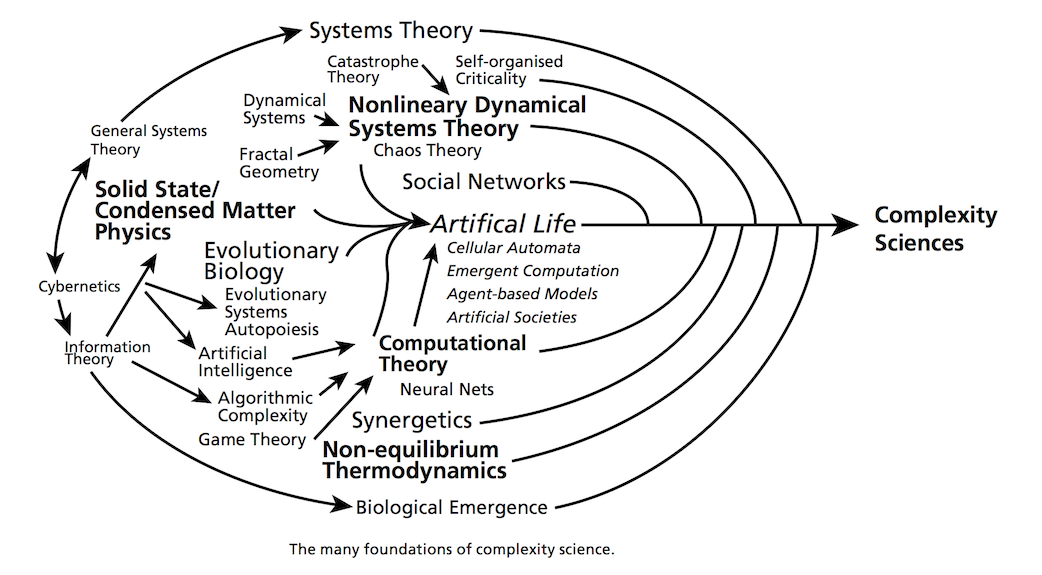
\includegraphics[width=0.99\linewidth]{images/foundations} \end{center}

\part{Preface}\label{part-preface}

\chapter*{\texorpdfstring{\textbf{Course
guide}}{Course guide}}\label{course-guide}
\addcontentsline{toc}{chapter}{\textbf{Course guide}}

Complexity research transcends the boundaries between the classical
scientific disciplines and is a hot topic in physics, mathematics,
biology, economy as well as psychology and the life sciences and is
collectively referred to as the Complexity Sciences. This course will
discuss techniques that allow for the study of human behaviour from the
perspective of the Complexity Sciences, specifically, the study of
complex physical systems that are alive and display complex adaptive
behaviour such as learning and development. Contrary to what the term
``complex'' might suggest, complexity research is often about finding
simple models / explanations that are able to simulate a wide range of
qualitatively different behavioural phenomena. ``Complex'' generally
refers to the object of study: Complex systems are composed of many
constituent parts that interact with one another across many different
temporal and spatial scales to generate behaviour at the level of the
system as a whole that can appear to be periodic, nonlinear, unstable or
extremely persistent. The focus of many research designs and analyses is
to quantify the degree of periodicity, nonlinearity, context sensitivity
or resistance to perturbation by exploiting the fact that ``everything
is interacting'' in complex systems. This requires a mathematical
formalism and rules of scientific inference that are very different from
the mathematics underlying traditional statistical analyses that assume
``everything is NOT interacting'' in order to be able to validly infer
statistical regularities in a dataset and generalise them to a
population. The complex systems approach to behavioural science often
overlaps with the idiographical approach of the science of the
individual, that is, the goal is not to generalise properties or
regularities to universal or statistical laws that hold at the level of
infinitely large populations, but to apply general principles and
universal laws that govern the adaptive behaviour of all complex systems
to study specific facts, about specific systems observed in specific
contexts at a specific instant.

The main focus of the course will be hands-on data-analysis and the main
analytical tool we will use is R (if you are an expert: It is also
possible to use Matlab for most of the assignments, let us know in
advance). Practical sessions will follow after a lecture session in
which a specific technique will be introduced.

We will cover the following topics:

\begin{itemize}
\tightlist
\item
  Theoretical background of phase transitions (self-organised
  criticality) and synchronisation (coupling dynamics) in complex
  dynamical systems and networks.
\item
  Simple models of linear and nonlinear dynamical behaviour (Linear \&
  logistic growth, Predator-Prey dynamics, Lorenz system, the chaos
  game);
\item
  Analysis of long range dependence in time and trial series (Entropy,
  Relative roughness, Standardized Dispersion Analysis, Detrended
  Fluctuation Analysis).
\item
  Quantification of temporal patterns in time and trial series including
  dyadic interactions (Phase Space Reconstruction, {[}Cross{]}
  Recurrence Quantification Analysis).
\item
  Network analyses (Estimating symptom networks, calculating network
  based complexity measures)
\end{itemize}

\section*{Teaching formats}\label{teaching-formats}
\addcontentsline{toc}{section}{Teaching formats}

Each meeting starts with a lecture addressing the theoretical and
methodological backgrounds of the practical applications that will be
used in hands-on assignments during the practical sessions. Several
meetings include a part where guest lecturers discuss the use of one or
more techniques in their recent research.

\section*{Test information}\label{test-information}
\addcontentsline{toc}{section}{Test information}

Examination will be based on a final assignment and a check of
participation in weekly discussions on blackboard (the content of
contributions will not be evaluated). Specifically:

\begin{itemize}
\tightlist
\item
  To prepare for each lecture students read a contemporary research
  paper in which a complex systems approach is used to a phenomenon
  studied in behavioural science. Students are required to formulate
  questions about each paper, and to initiate a discussion with their
  fellow-students on Blackboard. Each week at least one post by each
  student is expected in the discussion forum.
\item
  A final take-home assignment will be provided at the end of the
  course. Details will be discussed during the course. In general, the
  assignment will take about 2 days to complete, the time available to
  complete the assignment will be 1-2 weeks depending on the schedule.
\end{itemize}

This course is for students of the Research Master Behavioural Science.
Other Research Master students and PhD students interested in following
the course ask for permission by emailing to
\href{mailto:rm@bsi.ru.nl}{\nolinkurl{rm@bsi.ru.nl}} until 3 weeks
before the start of the course.

If permission is granted, this will be emailed 2 weeks before the start
of the course. Please confirm this mail! PhD students (RU and external)
have to subscribe through
\url{http://www.ru.nl/socialewetenschappen/onderwijs/overig/aanschuifonderwijs}
This course is not available for Bachelor and Master students.

\section*{Learning objectives
(specific)}\label{learning-objectives-specific}
\addcontentsline{toc}{section}{Learning objectives (specific)}

Students who followed this course will be able to:

\begin{itemize}
\tightlist
\item
  Critically evaluate whether their scientific inquiries can benefit
  from adopting theories, models, methods and analyses that were
  developed in the Complexity Sciences to study the structure and
  behaviour of complex adaptive systems.
\item
  Understand the differences between using an
  independent-statistical-component-dominant causal ontology, versus an
  interdependent-dynamical-interaction-dominant approach to the
  scientific study of human behaviour.
\item
  Understand and apply important terms to describe behavioural change
  and adaptation: Nonlinear dynamics (e.g.~hysteresis), attractor state,
  order parameter, control parameter, state-space, phase-space, phase
  transition, self-organisation, emergence, synergies as coordinative
  structures.
\item
  Simulate linear, nonlinear and coupled growth using simple
  mathematical models in Excel and R (or Matlab).
\item
  Fit parameters of simple models of linear and nonlinear growth to real
  data in SPSS or R (or Matlab).
\item
  Perform analyses on time and trial series of human performance and
  physiology that quantify the presence and nature of scaling relations
  (fractal geometry) in continuous or categorical data in R (or Matlab).
\item
  Perform analyses on time and trial series of human performance and
  physiology that quantify the presence and nature of temporal patterns
  (recurrent trajectories in phase space) in continuous or categorical
  data data in R (or Matlab).
\item
  Perform network analyses on datasets that may be considered static or
  dynamical representations of social networks, or symptom networks
  (psychopathology) in R.
\item
  Understand the results from analyses in terms of early warning signals
  indicating a phase transition might be imminent.
\item
  Understand the results from analyses in terms of synchronisation and
  coupling phenomena, e.g. ``complexity matching'' and
  ``leading/following'' behaviour.
\end{itemize}

\section*{learning goals (general)}\label{learning-goals-general}
\addcontentsline{toc}{section}{learning goals (general)}

At the end of this course, students have reached a level of
understanding that will allow them to:

\begin{itemize}
\tightlist
\item
  Study relevant scientific literature using a complex systems approach
  to behavioural science.
\item
  Getting help with using a complex systems approach in their own
  scientific inquiries, e.g.~by being able to ask relevant questions to
  experts on a specific topic discussed during the course.
\item
  Work through tutorials on more advanced topics that were not discussed
  during the course.
\item
  Keep up with the continuous influx of new theoretical, methodological
  and empirical studies on applying the complex systems approach in the
  behavioural-, cognitive- and neurosciences.
\end{itemize}

\subsection*{Preparation}\label{preparation}
\addcontentsline{toc}{subsection}{Preparation}

To prepare for each lecture students read a contemporary research paper
or watch a videolecture (e.g., \href{http://www.ted.com}{TED}) featuring
complexity theory and its application on a topic in behavioural science
that will be discussed in the subsequent lecture. Students are required
to formulate questions about each paper, and to initiate a discussion
with their fellow-students on Blackboard.

Before each lecture, students should:

\begin{itemize}
\tightlist
\item
  Read (parts of) a scientific article, or watch a videolecture
  featuring a complex systems perspective and/or methodology.
\item
  Ask (or answer) a question about what they have read / seen in the
  appropriate discussion forum on Blackboard.

  \begin{itemize}
  \tightlist
  \item
    The answers students provide will be discussed during the lecture.
  \end{itemize}
\end{itemize}

\section*{Literature}\label{literature}
\addcontentsline{toc}{section}{Literature}

Main literature:

\begin{itemize}
\tightlist
\item
  Hasselman, F., \& Wijnants, M. (2018). A Complex Systems Approach to
  the Behavioural Sciences. a practical guide to basic theory, models,
  methods and analyses {[}this book{]}
\item
  Rose, T. (2016). The end of average: How we succeed in a world that
  values sameness. Penguin UK. {[}also available in Dutch and many other
  languages{]}
\end{itemize}

Selected chapters from these books will be made available to make a
personal copy:

\begin{itemize}
\tightlist
\item
  Friedenberg, J. (2009). Dynamical psychology: Complexity,
  self-organization and mind. ISCE Publishing.
\item
  Kaplan, D., \& Glass, L. (2012). Understanding nonlinear dynamics.
  Springer Science \& Business Media.
\end{itemize}

A list of required and optional literature related to the topic
discussed in each session will be available on Blackboard.

\section{Schedule}\label{schedule}

The dates and locations can be found below. All lectures are on Thursday
from \texttt{10.45} to \texttt{12.30}. The practical sessions take place
on Thursday from \texttt{13.45} to \texttt{15.30}.

\section{\texorpdfstring{We use \texttt{R}!}{We use R!}}\label{we-use-r}

This text was transformed to \texttt{HTML}, \texttt{PDF} en
\texttt{ePUB} using \texttt{bookdown}\citep{R-bookdown} in
\href{https://www.rstudio.com}{\textbf{RStudio}}, the graphical user
interface of the statistical language
\href{https://www.r-project.org}{\textbf{R}} \citep{R-base}.
\texttt{bookdown} makes use of the \texttt{R} version of
\href{https://en.wikipedia.org/wiki/Markdown}{markdown} called
\href{http://rmarkdown.rstudio.com}{Rmarkdown} \citep{R-rmarkdown},
together with \href{http://yihui.name/knitr/}{knitr} \citep{R-knitr} and
\href{http://pandoc.org}{pandoc}.

We'll use some web applications made in
\href{http://shiny.rstudio.com}{Shiny} \citep{R-shiny}

Other \texttt{R} packages used are: \texttt{DT} \citep{R-DT},
\texttt{htmlTable} \citep{R-htmlTable}, \texttt{plyr} \citep{R-plyr},
\texttt{dplyr} \citep{R-dplyr},\texttt{tidyr} \citep{R-tidyr},
\texttt{png} \citep{R-png}, \texttt{rio} \citep{R-rio}.

\chapter{Introduction}\label{intro}

You can label chapter and section titles using \texttt{\{\#label\}}
after them, e.g., we can reference Chapter \ref{intro}. If you do not
manually label them, there will be automatic labels anyway, e.g.,
Chapter \ref{methods}.

Figures and tables with captions will be placed in \texttt{figure} and
\texttt{table} environments, respectively.

\begin{Shaded}
\begin{Highlighting}[]
\KeywordTok{par}\NormalTok{(}\DataTypeTok{mar =} \KeywordTok{c}\NormalTok{(}\DecValTok{4}\NormalTok{, }\DecValTok{4}\NormalTok{, .}\DecValTok{1}\NormalTok{, .}\DecValTok{1}\NormalTok{))}
\KeywordTok{plot}\NormalTok{(pressure, }\DataTypeTok{type =} \StringTok{'b'}\NormalTok{, }\DataTypeTok{pch =} \DecValTok{19}\NormalTok{)}
\end{Highlighting}
\end{Shaded}

\begin{figure}

{\centering 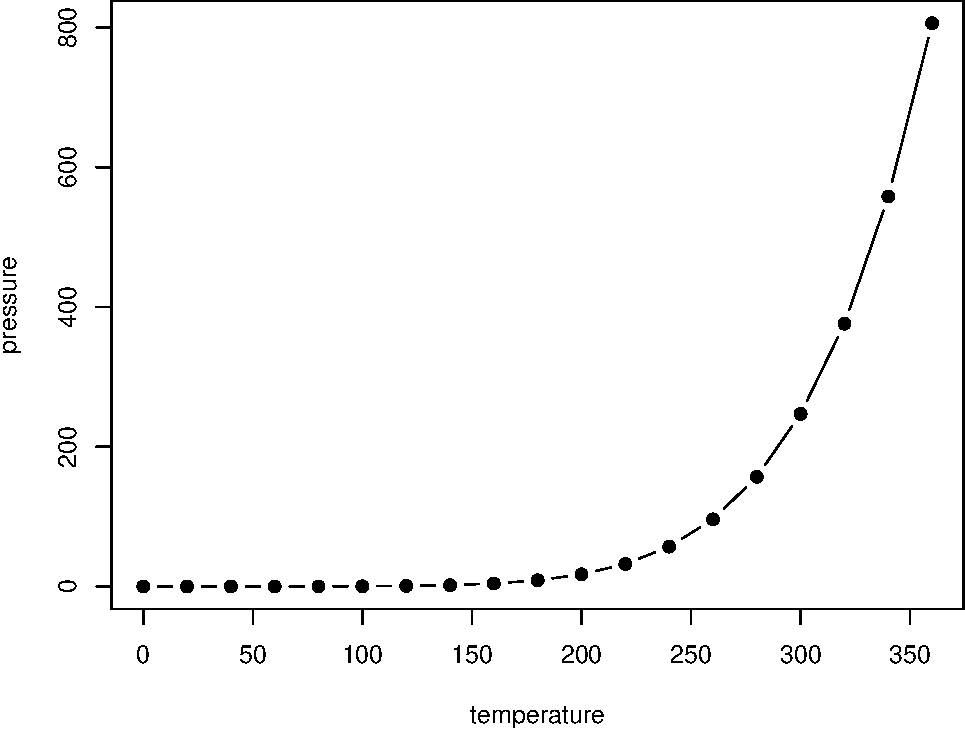
\includegraphics[width=0.8\linewidth]{DCS1718_files/figure-latex/nice-fig-1} 

}

\caption{Here is a nice figure!}\label{fig:nice-fig}
\end{figure}

Reference a figure by its code chunk label with the \texttt{fig:}
prefix, e.g., see Figure \ref{fig:nice-fig}. Similarly, you can
reference tables generated from \texttt{knitr::kable()}, e.g., see Table
\ref{tab:nice-tab}.

\begin{Shaded}
\begin{Highlighting}[]
\NormalTok{knitr}\OperatorTok{::}\KeywordTok{kable}\NormalTok{(}
  \KeywordTok{head}\NormalTok{(iris, }\DecValTok{20}\NormalTok{), }\DataTypeTok{caption =} \StringTok{'Here is a nice table!'}\NormalTok{,}
  \DataTypeTok{booktabs =} \OtherTok{TRUE}
\NormalTok{)}
\end{Highlighting}
\end{Shaded}

\begin{table}

\caption{\label{tab:nice-tab}Here is a nice table!}
\centering
\begin{tabular}[t]{rrrrl}
\toprule
Sepal.Length & Sepal.Width & Petal.Length & Petal.Width & Species\\
\midrule
5.1 & 3.5 & 1.4 & 0.2 & setosa\\
4.9 & 3.0 & 1.4 & 0.2 & setosa\\
4.7 & 3.2 & 1.3 & 0.2 & setosa\\
4.6 & 3.1 & 1.5 & 0.2 & setosa\\
5.0 & 3.6 & 1.4 & 0.2 & setosa\\
\addlinespace
5.4 & 3.9 & 1.7 & 0.4 & setosa\\
4.6 & 3.4 & 1.4 & 0.3 & setosa\\
5.0 & 3.4 & 1.5 & 0.2 & setosa\\
4.4 & 2.9 & 1.4 & 0.2 & setosa\\
4.9 & 3.1 & 1.5 & 0.1 & setosa\\
\addlinespace
5.4 & 3.7 & 1.5 & 0.2 & setosa\\
4.8 & 3.4 & 1.6 & 0.2 & setosa\\
4.8 & 3.0 & 1.4 & 0.1 & setosa\\
4.3 & 3.0 & 1.1 & 0.1 & setosa\\
5.8 & 4.0 & 1.2 & 0.2 & setosa\\
\addlinespace
5.7 & 4.4 & 1.5 & 0.4 & setosa\\
5.4 & 3.9 & 1.3 & 0.4 & setosa\\
5.1 & 3.5 & 1.4 & 0.3 & setosa\\
5.7 & 3.8 & 1.7 & 0.3 & setosa\\
5.1 & 3.8 & 1.5 & 0.3 & setosa\\
\bottomrule
\end{tabular}
\end{table}

You can write citations, too. For example, we are using the
\textbf{bookdown} package \citep{R-bookdown} in this sample book, which
was built on top of R Markdown and \textbf{knitr} \citep{xie2015}.

\part{Mathematics of
Change}\label{part-mathematics-of-change}

\chapter*{\texorpdfstring{\textbf{Modeling 1 Dimensional Change
Processes}}{Modeling 1 Dimensional Change Processes}}\label{modeling-1-dimensional-change-processes}
\addcontentsline{toc}{chapter}{\textbf{Modeling 1 Dimensional Change
Processes}}

The simplest non-trivial \emph{iterative change process} can be
described by the following \emph{difference equation}:

\[ Y_{t+1} = Y_{t=0} + a*Y_t \]

The equation describes the way in which the value of \(Y\) changes
\href{https://en.wikipedia.org/wiki/Discrete_time_and_continuous_time}{between
two adjacent, discrete moments in time} (hence the term
\href{https://en.wikipedia.org/wiki/Recurrence_relation}{difference
equation, or recurrence relation}). There are two parameters resembling
an intercept and a slope:

\begin{enumerate}
\def\labelenumi{\arabic{enumi}.}
\tightlist
\item
  The starting value \(Y_0\) at \(t=0\), also called the \emph{starting
  value}, or the \emph{initial conditions}.
\item
  A rule for incrementing time, here the change in \(Y\) takes place
  over a discrete time step of 1: \(t+1\).
\end{enumerate}

The values taken on by variable \(Y\) are considered to represent the
states quantifiable observable leAlternative ways to describe the change
of states :

\begin{itemize}
\tightlist
\item
  A dynamical rule describing the propagation of the states of a system
  observable measured by the values of variable \texttt{Y} through
  discrete time.
\item
  A dynamic law describing the time-evolution of the states of a system
  observable measured by the variable \texttt{Y}.
\end{itemize}

These descriptions all refer to the change processes that govern system
observables (properties of dynamical systems that can be observed
through measurement).

\section*{\texorpdfstring{\textbf{It's a line! It's a
plane!}}{It's a line! It's a plane!}}\label{its-a-line-its-a-plane}
\addcontentsline{toc}{section}{\textbf{It's a line! It's a plane!}}

The formula resembles the equation of a line. There is a constant value
\(Y_{0}\) which is added to a proportion of the value of \(Y\) at time
\(t\), given by parameter \(a\). This is equivalent to the slope of a
line. However, in a \((X,Y)\) plane there are two `spatial' (metric)
dimensions representing the values two variables \(X\) and \(Y\) can
take on (see figure).

\begin{center}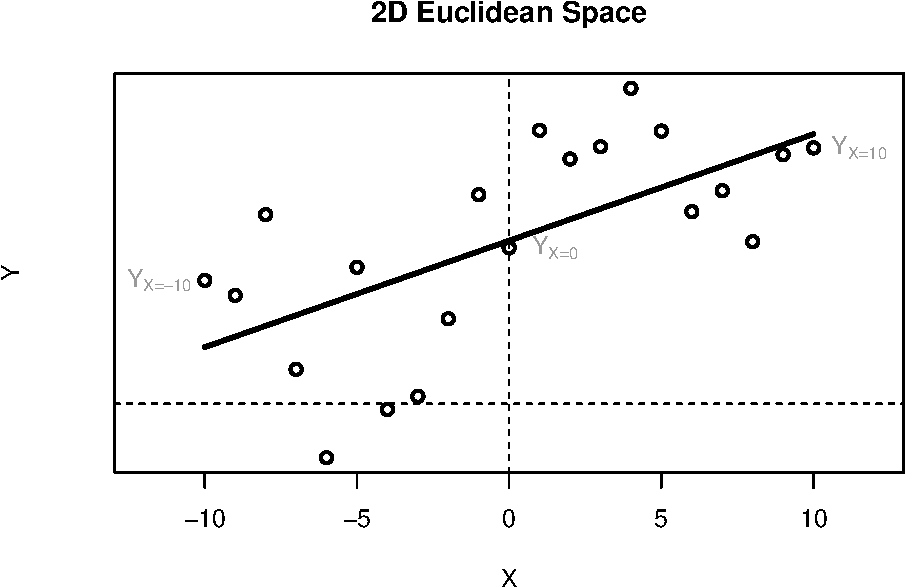
\includegraphics[width=0.99\linewidth]{DCS1718_files/figure-latex/unnamed-chunk-1-1} \end{center}

The best fitting straight line would be called a statistical model of
the linear relationship between the observed values of \(X\) and \(Y\).
It can be obtained by fitting a General Linear Model (GLM) to the data.
If \(X\) were to represent repeated measurements the multivariate GLM
for repeated measures would have to be fitted to the data. This can be
very problematic, because statistical models rely on
\href{https://en.wikipedia.org/wiki/Ergodic_theory}{Ergodic theory}:

\begin{quote}
``\ldots{} it is the study of the long term average behavior of systems
evolving in time.'' \footnote{See Dajani \& Dirksin (2008, p.~5,
  \href{http://www.staff.science.uu.nl/~kraai101/lecturenotes2009.pdf}{``A
  simple introduction to Ergodic Theory''})}
\end{quote}

need to assume independence of measurements within and between subjects.
These assumptions can be translated to certain conditions that must hold
for the model to be valid, known as \emph{Compound Symmetry} and
\emph{Sphericity}:

\begin{quote}
The compound symmetry assumption requires that the variances (pooled
within-group) and covariances (across subjects) of the different
repeated measures are homogeneous (identical). This is a sufficient
condition for the univariate F test for repeated measures to be valid
(i.e., for the reported F values to actually follow the F distribution).
However, it is not a necessary condition. The sphericity assumption is a
necessary and sufficient condition for the F test to be valid; it states
that the within-subject ``model'' consists of independent (orthogonal)
components. The nature of these assumptions, and the effects of
violations are usually not well-described in ANOVA textbooks; \footnote{\href{https://www.statsoft.com/Textbook/ANOVA-MANOVA\#sphericity}{Retreived
  from www.statsoft.com}}
\end{quote}

As you can read in the quoted text above, these conditions must hold in
order to be able to identify unique independent components as the
sources of variation of \(Y\) over time within a subject. This is the a
clear example of:

\begin{quote}
It is the theory that decides what we may observe \footnote{Einstein as
  quoted by Heisenberg.}
\end{quote}

If you choose to use GLM repeated measures to model change over time,
you will only be able to infer independent components that are
responsible for the time-evolution of \(Y\). As is hinted in the last
sentence of the quote, the validity of such inferences is not a common
topic of discussion statistics textbooks.

\section*{\texorpdfstring{\textbf{No! \ldots{} It's a
\href{https://en.wikipedia.org/wiki/Time_series}{time
series}!}}{No! \ldots{} It's a time series!}}\label{no-its-a-time-series}
\addcontentsline{toc}{section}{\textbf{No! \ldots{} It's a
\href{https://en.wikipedia.org/wiki/Time_series}{time series}!}}

The important difference between a regular 2-dimensional Euclidean plane
and the space in which we model change processes is that the \(X\)-axis
represents the physical dimension \textbf{time}. In the case of the
Linear Map we have a 1D space with one `spatial' dimension \(Y\) and a
time dimension \(t\). This is called time series if \(Y\) is sampled as
a continuous process, or a trial series if the time between subsequent
observations is not relevant, just the fact that there was a temporal
order (for example, a series of response latencies to trials in a
psychological experiment in the order in which they were presented to
the subject).

\begin{center}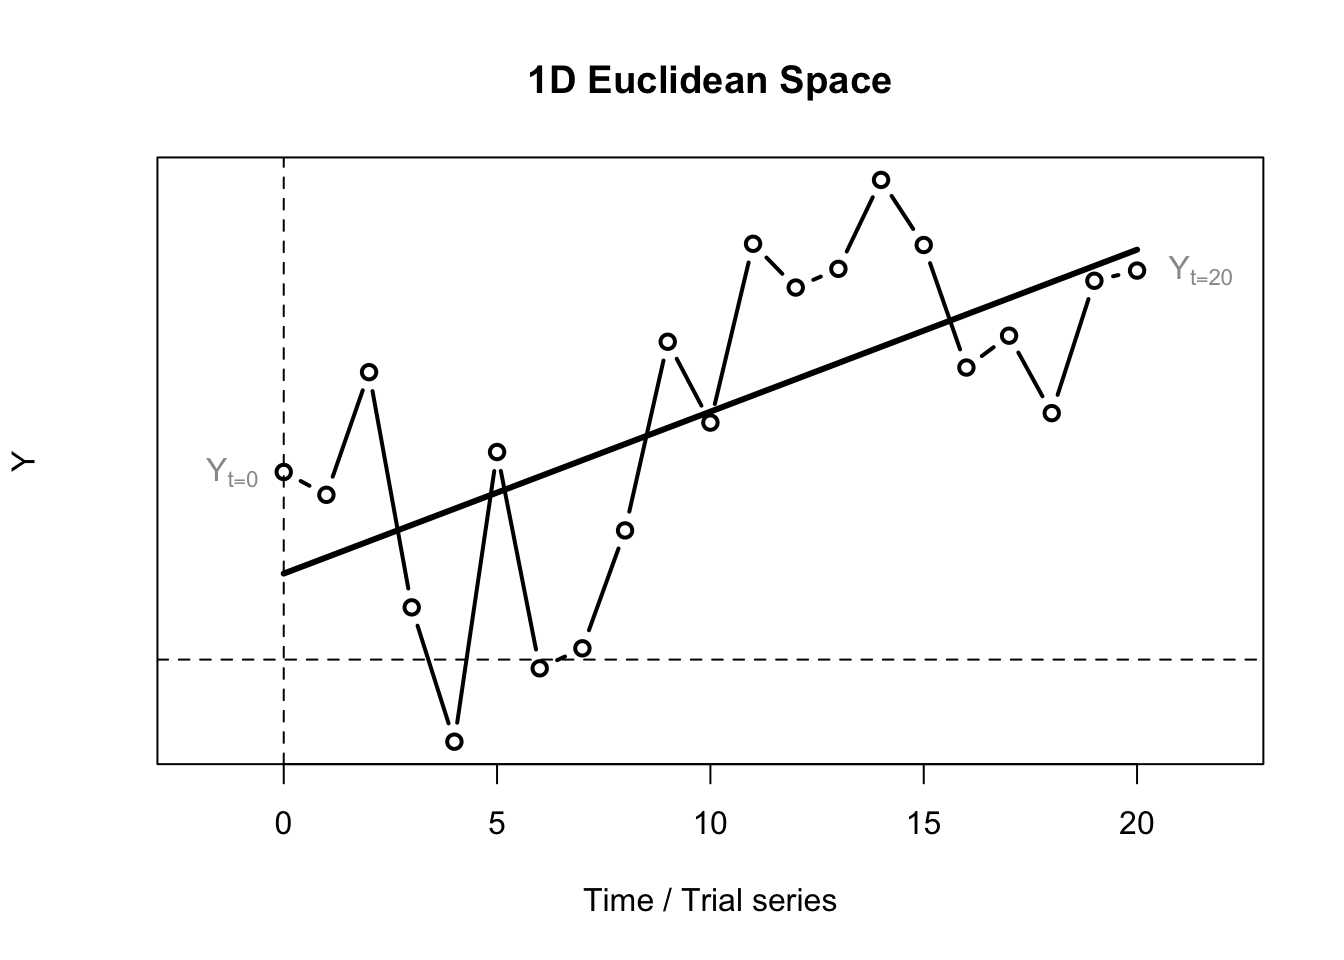
\includegraphics[width=0.99\linewidth]{DCS1718_files/figure-latex/unnamed-chunk-2-1} \end{center}

Time behaves different from a spatial dimension in that it is
directional (time cannot be reversed), it cannot take on negative
values, and, unless one is dealing with a truly random process, there
will be a temporal correlation across one or more values of \(Y\)
seperated by an amount of time. In the linear difference equation this
occurs because each value one step in the future is calculated based on
the current value. If the values of \(Y\) represent an observable of a
dynamical system, the system can be said to have a history, or a memory.
Ergodic systems do not have a history or a memory that extends across
more than one time step. This is very convenient, because one can
calculate the expected value of a system observable given infinite time,
by making use of of the laws of probabilities of random events (or
random fields). This means: The average of an observable of an Ergodic
system measured across infinite time (its entire history, the
\textbf{time-average}), will be the be the same value as the average of
this observable measured at one instance in time, but in an infinite
amount of systems of the same kind (the population, the \textbf{spatial
average}) \footnote{In other words: If you throw 1 die 100 times in a
  row, the average of the 100 numbers is the \textbf{time-average} of
  one of the observables of die-throwing systems. If this system is
  ergodic, then its \textbf{time-average} is expected to be similar to
  the average of the numbers that turn up if you throw 100 dice all at
  the same instance of time. The dice layed out on the table represent a
  spatial sample, a snapshot frozen in time, of the possible states the
  system can be in. Taking the average would be the \textbf{spatial
  average} this observable of die-throwing systems. This ergodic
  condiciotn is often implicitly assumed in Behavioural Science when
  studies claim to study change by taking different samples of
  individuals (snapshots of system states) and comparing if they are the
  same.}.

The simple linear difference equation will have a form of *perfect
memory' across the smallest time scale (i.e., the increment of 1,
\(t+1\)). This `memory' concerns a correlation of 1 between values at
adjacent time points (a short range temporal correlation, SRC), because
the change from \(Y_t\) to \(Y_{t+1}\) is exactly equal to \(a * Y_t\)
at each iteration step. This is the meaning of deterministic, not that
each value of \(Y\) is the same, but that the value of \(Y\) now can be
perfectly explained form the value of \(Y\) one moment in the past.

Summarising, the most profound difference is not the fact that the
equation of linear change is a deterministic model and the GLM is a
probabilistic model with parameters fitted from data, this is something
we can (and will) do for \(a\) as well. The profound difference between
the models is the role given to the passage of time:

\begin{itemize}
\tightlist
\item
  The linear difference equation represents changes in \(Y\) as a
  function of the physical dimension \emph{time} and \(Y\) itself.
\item
  The GLM represents changes in \(Y\) as a function of a
  \href{https://en.wikipedia.org/wiki/Linear_predictor_function}{linear
  predictor} composed of additive components that can be regarded as
  independent sources of variation that sum up to the observed values of
  \(Y\).
\end{itemize}

\begin{center}\rule{0.5\linewidth}{\linethickness}\end{center}

\chapter{Methods}\label{methods}

We describe our methods in this chapter.

\chapter{Applications}\label{applications}

Some \emph{significant} applications are demonstrated in this chapter.

\section{Example one}\label{example-one}

\section{Example two}\label{example-two}

\chapter{Final Words}\label{final-words}

We have finished a nice book.

\chapter{Final Words}\label{final-words-1}

We have finished a nice book.

\chapter{Final Words}\label{final-words-2}

We have finished a nice book.

\chapter{Final Words}\label{final-words-3}

We have finished a nice book.

\bibliography{book.bib}


\end{document}
